\documentclass[12pt]{article}
\title{3D Software Rasterisation Renderer \\ \large Com S 424 Final Project}
\author{Ian Malerich \\ imm@iastate.edu}
\usepackage{amssymb, amsfonts, amsthm, mathtools, graphicx, breqn}
\usepackage{minted, subfig, float, scrextend, setspace, soul, caption, subcaption}
\usemintedstyle{friendly}
\usepackage[hidelinks]{hyperref}

\onehalfspacing
\begin{document}

\maketitle

\section*{Introduction}

This project implements a rendering system for 3 dimensional graphics, defined as a set
of triangles in 3 dimensional space. Models are input via a .obj file containing triangle data
as well as a .mtl referenced by the .obj file which holds texture information. A camera is set
at the origin looking down the z-axis and captures a single image representing the scene.
Therefore the problem size varies across two primary variables: the number of triangles which
need to be rendered and the dimensions of the output texture, that is, how many pixel need
to be colored.

\bigbreak
\begin{center}
	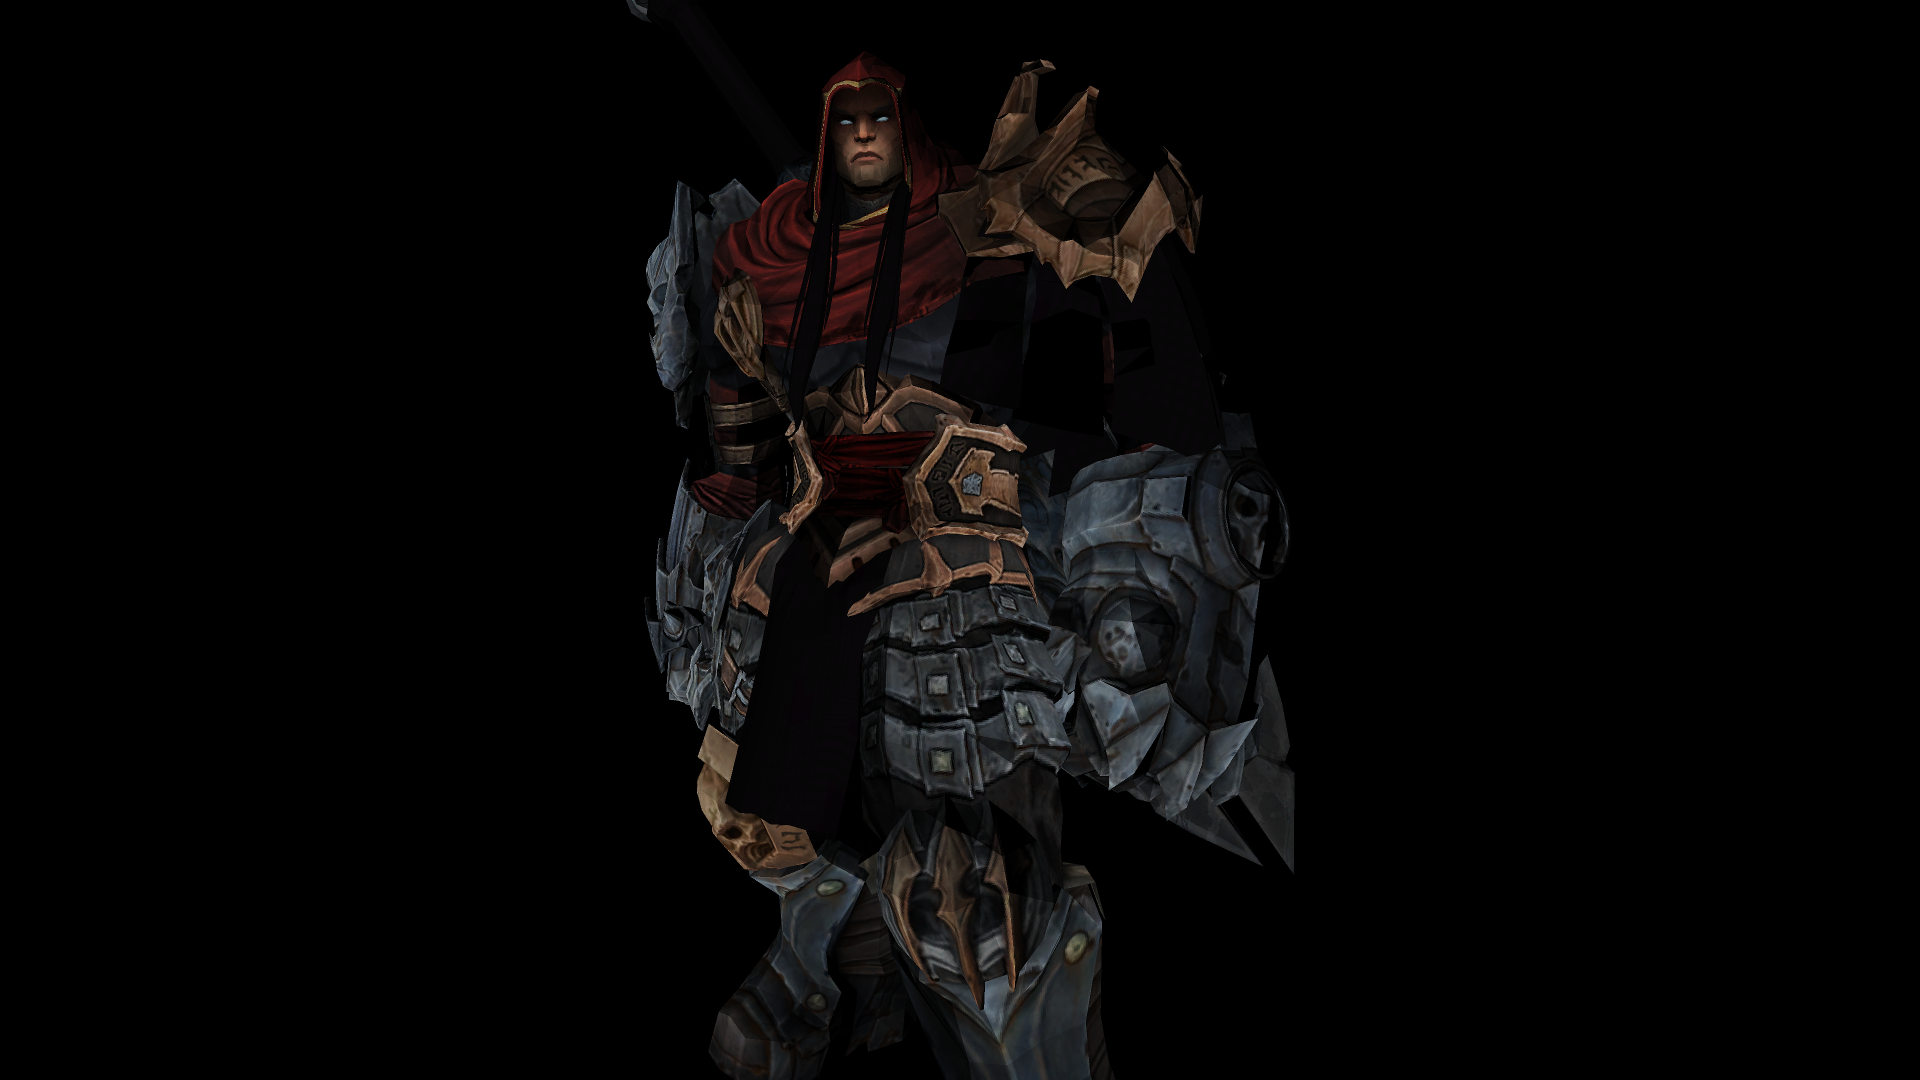
\includegraphics[scale=0.13]{war.png}
\end{center}

\clearpage
\section*{Systems}

Results are included for both my personal system and the hpc cluster. The below chart provides some basic
information about each system as read from /proc/cpuinfo.

\bigbreak
\begin{center}
	\begin{tabular}{|l|c|c|}
		\hline
		system & personal & hpc-class \\ \hline \hline
		model name & i7-3630QM & Xeon CPU-E5-2650 \\ \hline
		cores & 4 & 8 \\ \hline
		processors & 8 & 16 \\ \hline
		clock speed & 2.40GHz & 2.00GHz \\ \hline
		cache size & 6144 KB & 20480 KB \\ \hline
		address size (physical) & 36 bits & 46 bits \\ \hline
		address size (virtual) & 48 bits & 48 bits \\ \hline
	\end{tabular}
\end{center}

\section*{Models}

Below are a list of models which will be used for various performance tests as well as how many
vertices make up the model. Note that each model has accompanying textures which will affect memory
usage but in terms of performance texture samples are handled per pixel and thus the output image
size is the bigger concern and not buffer size.
It is worth mentioning that while the model 'war' has the least vertices, it is the only model
not made up of a single mesh. Rather, war is made up by 10 smaller models each with their own texture.
Thus as the provided graphs will demonstrate the performance of this mesh does not quite fall in line
with the other models.

\begin{center}
	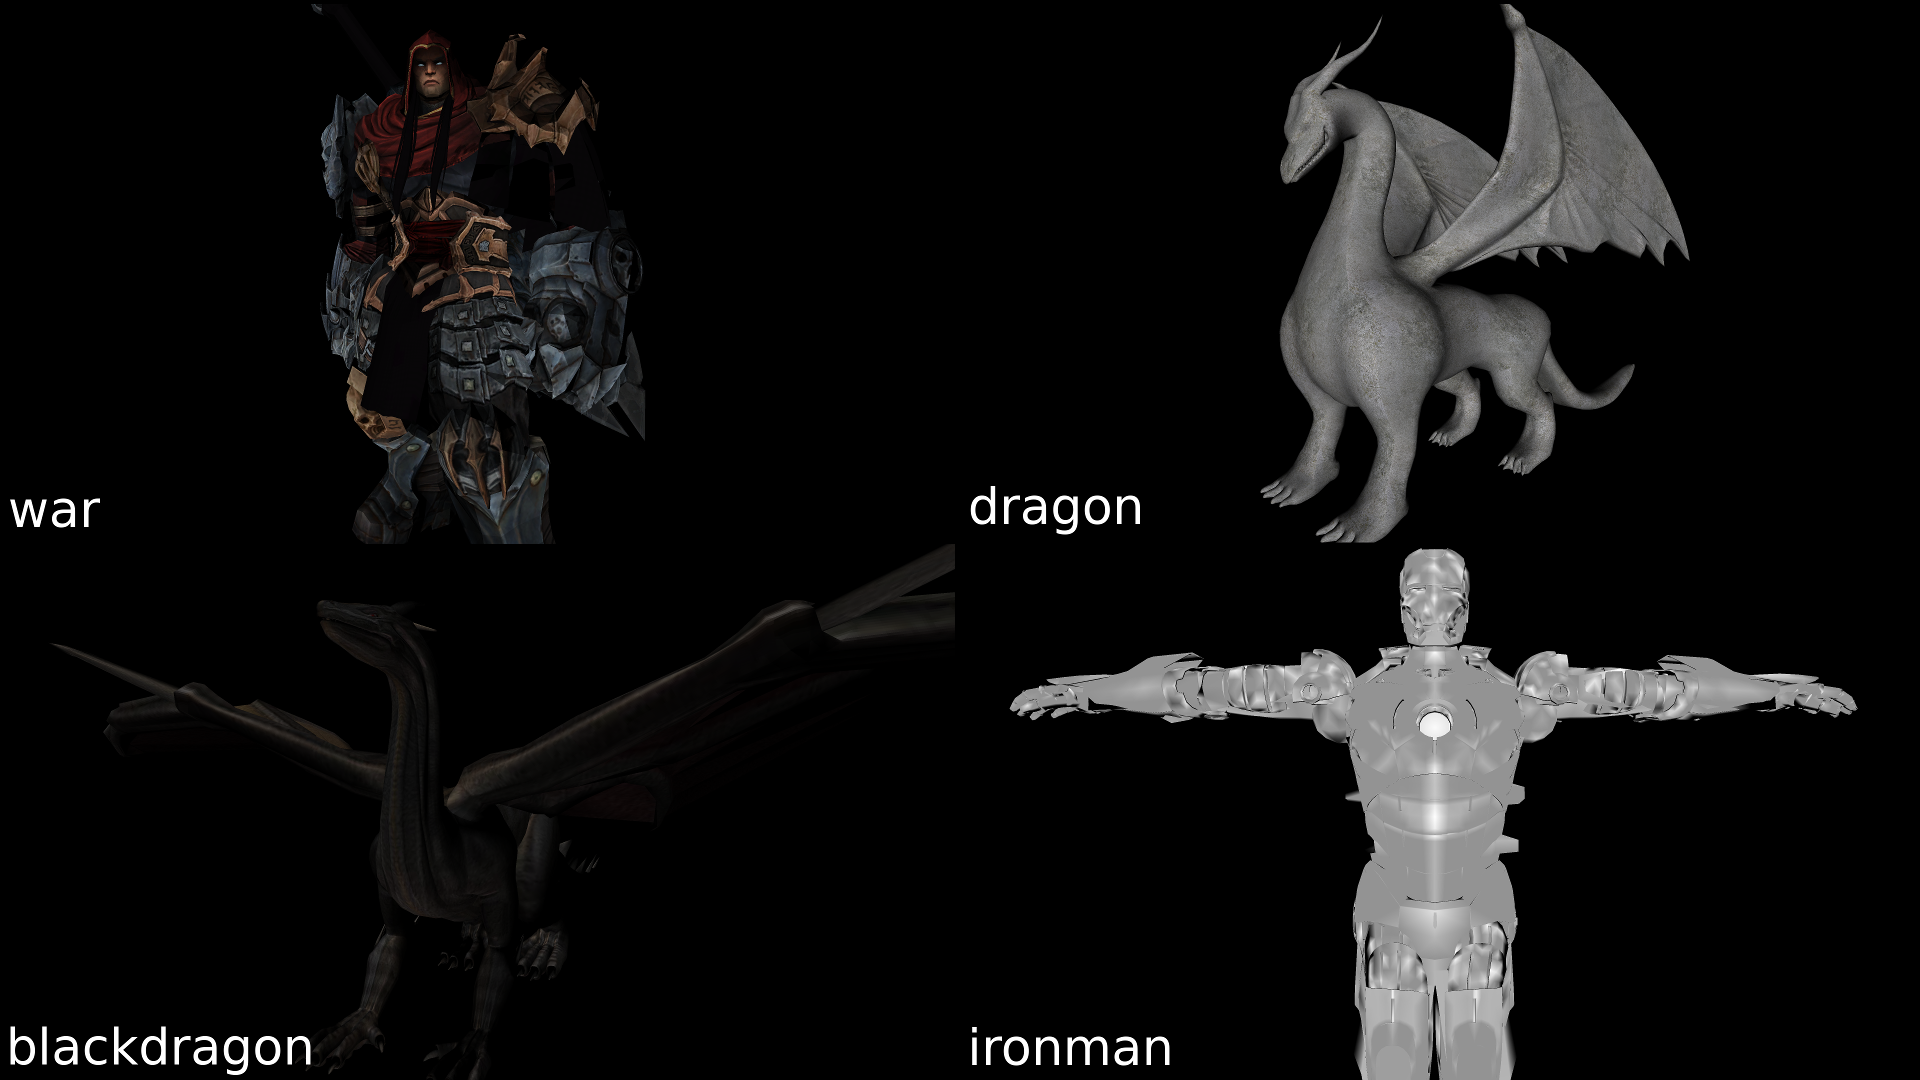
\includegraphics[scale=0.225]{models.png}
\end{center}

\bigbreak
\begin{center}
	\begin{tabular}{|l|c|c|}
		\hline
		name & vertex count & parts \\ \hline \hline
		war & 44,115 & 10 \\ \hline
		dragon & 61,152 & 1 \\ \hline
		blackdragon & 113,955 & 1 \\ \hline
		iron man & 596,682 & 1 \\ \hline
	\end{tabular}
\end{center}

\section*{Performance}

The primary goal in regards to performance is to minimize total rendering time. To that respect, I will
not be including model and texture load times as well as output image write time in any measurements. 
In a later section I will provide a brief look at memory usage, however due to the nature of the project, a
large amount of memory will be held by model and texture buffers which will dwarf the added memory requirements
of multi-threading in OpenMP.

\section*{Serial Execution}

Below we can see how well my code performs when running in serial. We can clearly see that the output
image resolution has a much greater influence on total render time. Number of vertices does tend to
produce longer render times but the increase is much more gradual. Note that an output image of 
size $3840x2160$ (orange) is exactly $4\times$ that of $1920x1080$ (blue) thus based only on results so far
render time appears to scale almost linearly with image resolution.

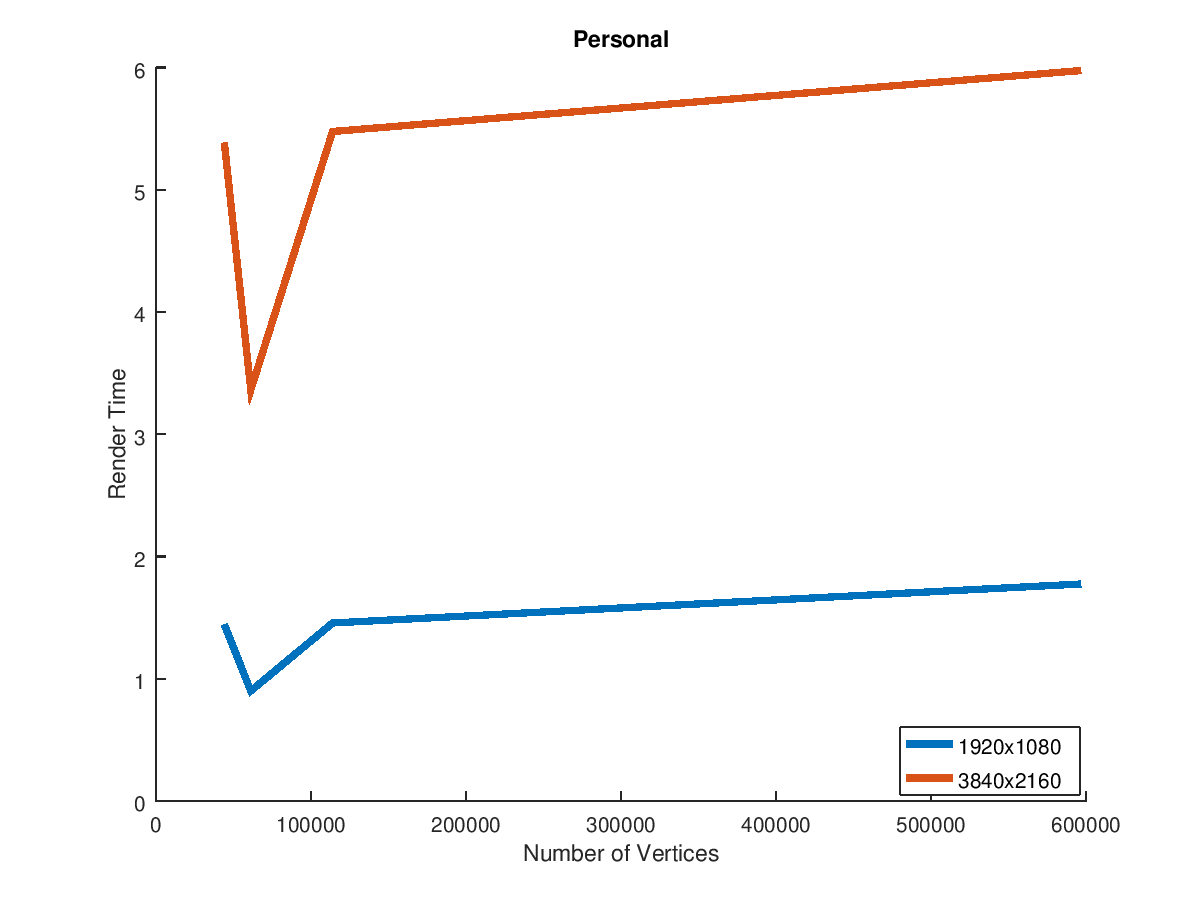
\includegraphics[scale=0.65]{serial_personal.png}

\section*{Parallelization}

The easiest method, and the first method I will try, to parallelize this code is a simple parallel for
directive loop over each face. Each thread will then transform 3 vertices corresponding to its assigned
face, and then draw the given triangle. Within the draw_triangle methoda critical sections are needed
when writing to the back and output buffers so that only one thread may write at a time. All other
operations may be performed in parallel.

\begin{minted}[linenos]{c}
for (unsigned k=0; k<models.model_count; k++) {
	model_t m = models.models[k];

	#pragma omp parallel for num_threads(thread_count)
	for (int i=0; i<num_faces(m); i++) {
		transform_vertex(&v[3*i + 0], proj, WIDTH, HEIGHT);
		transform_vertex(&v[3*i + 1], proj, WIDTH, HEIGHT);
		transform_vertex(&v[3*i + 2], proj, WIDTH, HEIGHT);

		draw_triangle(&m, i, simple_shader, 
			m.material, buffer, back_buffer, SIZE);
	}
}
\end{minted}
\textcolor[RGB]{200,200,200}{\rule{\textwidth}{0.75pt}}\bigbreak
\begin{minted}[linenos]{c}
	#pragma omp critical
	{
		if (back[y*buffer_size.x + x] > pos.z) {
			back[y*buffer_size.x + x] = pos.z;

			// interpolate vertex data
			vector_t tex_coord = interpolate(tex_coords, 
				bc_screen);
			vector_t norm = interpolate(norms, bc_screen);
			vector_t tan = interpolate(tans, bc_screen);

			vector_t c = shader((shader_data_t){pos, 
				tex_coord, norm, tan}, material);
			draw_point(vector_to_point(pos), 
				vector_to_color(c), buffer, buffer_size);
		}
	}
\end{minted}

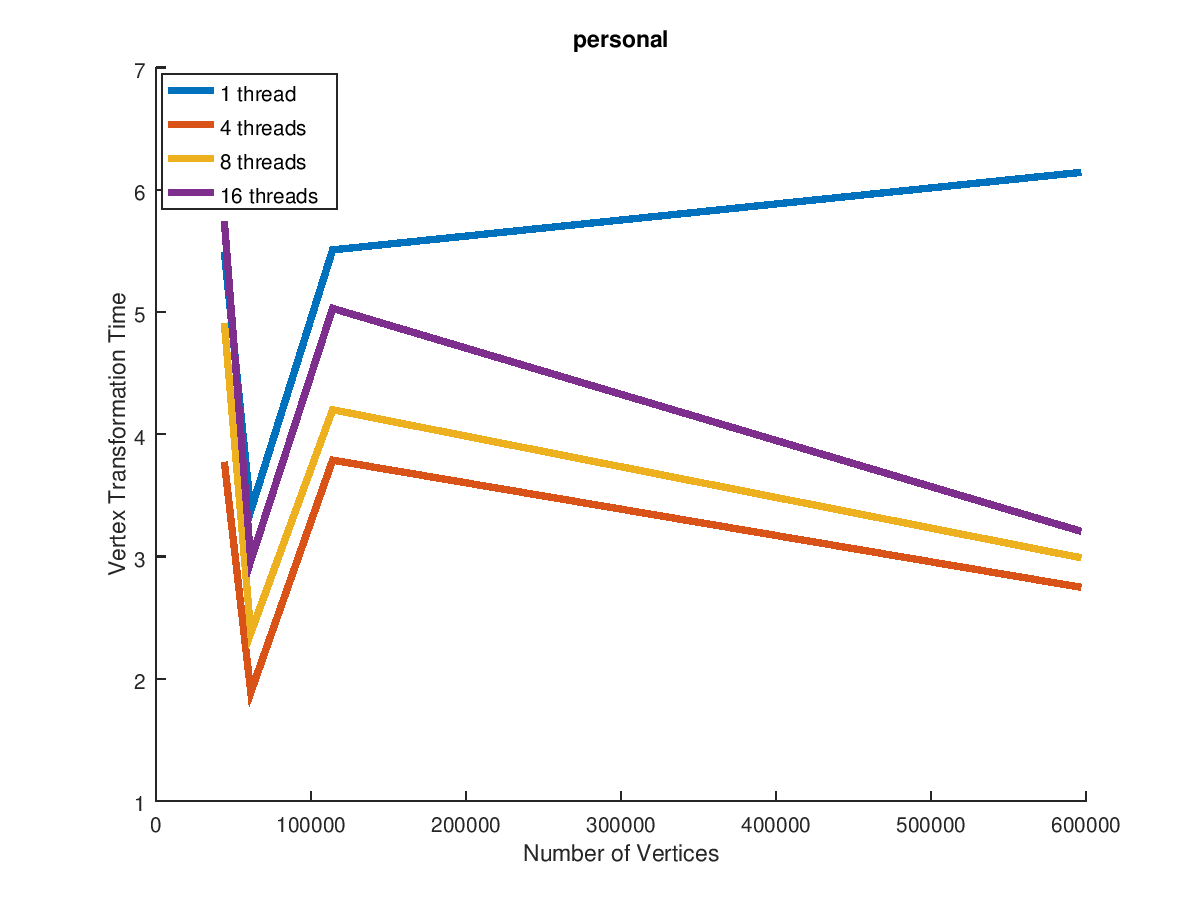
\includegraphics[scale=0.65]{parallel0_personal.png}

In this next approach I split the work of transforming vertices and rendering each triangle.
Each vertex can be parallelized on its own thread, as no vertex depends on another vertex. Since
we know that the majority of time is spent actually rasterising triangles I have commented that section
out, this will give me a better look at whether or not I am getting any benefit out of OpenMP for this
portion of code.

\begin{minted}[linenos]{c}
	for (unsigned k=0; k<models.model_count; k++) {
		model_t m = models.models[k];

		#pragma omp parallel for num_threads(16)
		for (unsigned i=0; i<m.vert_count; i++) {
			transform_vertex(&m.vertices[i], &proj, 
				WIDTH, HEIGHT);
		}

		// for (int i=0; i<num_faces(m); i++) {
		// 	draw_triangle(&m, i, simple_shader, m.material, 
		// 		buffer, back_buffer, SIZE);
		// }
	}
\end{minted}

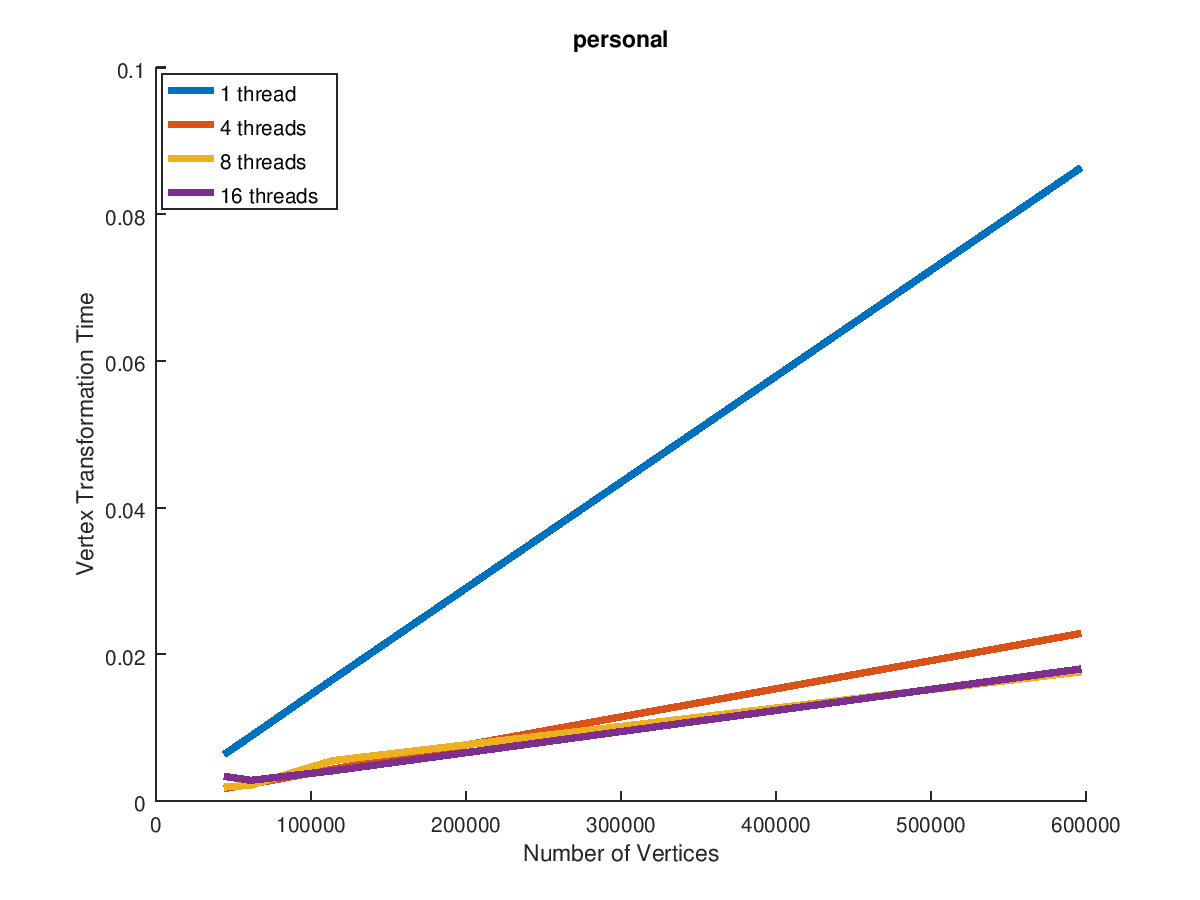
\includegraphics[scale=0.65]{parallel1_personal.png}

\section*{References}

\begin{itemize}
	\item Lengyel, Eric. \textit{Mathematics for 3D Game Programming and Computer Graphics.} Course Technology,
Cengage Learning, 2012.
	\item Sokolov, Dmitry. ``Tinyrenderer". \url{https://github.com/ssloy/tinyrenderer/wiki}
	\item Barrett, Sean. ``stb". \url{https://github.com/nothings/stb}
	\item Michael S\"uB and Claudia Leopold. \textit{Common Mistakes in OpenMP and How To Avoid Them}.
\end{itemize}

\end{document}
